\section{Introducción}
\subsection{Planteamiento del problema}

La robótica está cada vez más involucrada en el mercado laboral, lo que hace que la educación, en muchos casos, se quede corta para cubrir esta demanda. Por ello, se busca fomentar la inclusión de la robótica en diferentes niveles educativos: inspirando a los más jóvenes, introduciendo a los estudiantes en educación secundaria, y permitiendo que los más avanzados puedan profundizar en el área.

En este contexto, surge la necesidad de un modelo de brazo robótico accesible, fácil de ensamblar, de bajo costo y con un diseño sencillo que sea adecuado para usuarios inexpertos o jóvenes. Este modelo debe ser, además, duradero, mantenible y fácil de reparar, para garantizar su uso a largo plazo. Adicionalmente, se plantea que el manipulador sea modular, con la posibilidad de modificación y expansión, permitiendo a los estudiantes más avanzados involucrarse en proyectos más complejos y adaptarlos a otros sistemas o tecnologías.

La propuesta de utilizar MDF como material principal, aprovechando sus ventajas de bajo costo y facilidad de fabricación mediante corte láser o fresado CNC, busca superar las limitaciones que presentan los métodos de fabricación más lentos y costosos como la impresión 3D. De esta forma, se logra una producción más eficiente y replicable, accesible para más instituciones educativas.

El objetivo final es ofrecer un manipulador robótico que pueda adaptarse a diversas aplicaciones y demostraciones, fomentando el aprendizaje en robótica y automatización desde etapas tempranas de formación, inspirando a los estudiantes y acercándolos a los procesos industriales actuales.

\subsection{Diagrama de Ishikawa}

\vspace{1em}


\begin{figure}[h]
  \centering
  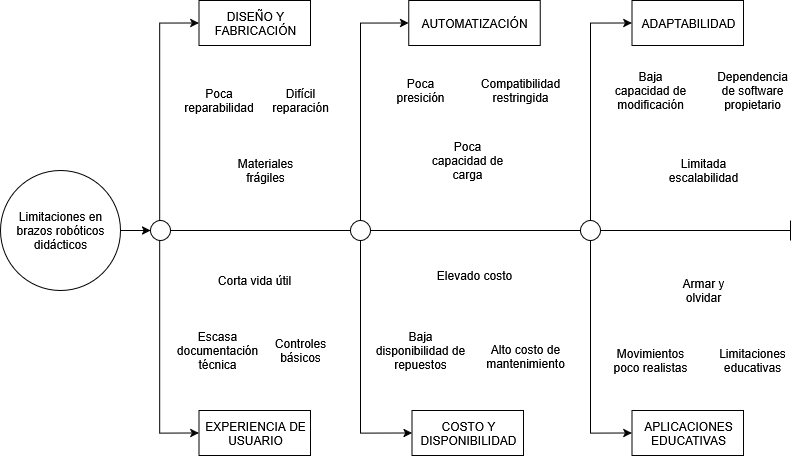
\includegraphics[width=0.8\textwidth]{anexos/Diagrama Ishikawa.png}
  \caption{Diagrama de Ishikawa (Fuente: elaboración propia)}\label{fig:Diagrama Ishikawa.}
\end{figure}
En el diagrama se identifican seis ramas principales que agrupan las limitaciones más comunes de los brazos robóticos didácticos disponibles en el mercado. Cada una de ellas aborda un conjunto de problemáticas específicas:
\begin{itemize}
  \item Diseño y fabricación: engloba aspectos relacionados con la construcción del brazo, los materiales empleados y la facilidad de reparación o mantenimiento.
  \item Automatización: considera las limitaciones en la precisión, capacidad de carga, compatibilidad y posibilidades de integración con otros sistemas de control.
  \item Adaptabilidad: se refiere a la capacidad de modificar, escalar o personalizar el brazo, así como a la dependencia de software propietario que restringe su flexibilidad.
  \item Experiencia de usuario: abarca las dificultades que enfrentan los usuarios en el manejo del brazo, tales como controles limitados, documentación insuficiente y vida útil reducida.
  \item Costo y disponibilidad: contempla el precio de adquisición, el costo de mantenimiento y la dificultad para conseguir repuestos o componentes compatibles.
  \item Aplicaciones educativas: analiza las limitaciones de los kits en contextos formativos, como la escasa realismo de los movimientos y el alcance reducido de sus usos pedagógicos.
\end{itemize}

\subsection{Solución propuesta}
Un brazo robótico didáctico a escala de 4 GDL con efector intercambiable: electroimán (para piezas ferromagnéticas) y garra (para piezas no magnéticas). Estructura paramétrica cortada en MDF (3.2–10 mm), tornillería estándar y electrónica de fácil reposición. Control con ESP32/ATmega328P, modos manual/automático, GUI en Python (Tkinter/PyQt), y documentación abierta para replicación.

\subsection{Objetivo General}
Diseñar, construir y validar un brazo robótico didáctico de 4 GDL, seguro, portable y de bajo costo, con efectores electroimán/garra intercambiables, capaz de ejecutar tareas básicas de pick \& place en un volumen de trabajo de hasta 50×50×50 cm.

\subsection{Objetivos específicos}
\begin{enumerate}
  \item \textbf{Repetibilidad:} $\leq$ 3--5\,mm en el volumen útil (validado con 10 repeticiones por punto).
  \item \textbf{Carga y alcance:} manipular $\leq$ 100\,g a un alcance de 40\,cm con tasa de éxito $\geq 90\%$ (10 intentos).
  \item \textbf{Tiempo de ciclo:} \emph{pick} $\rightarrow$ \emph{place} $\rightarrow$ retorno $\leq$ 3\,s a 10--15\,cm entre posiciones.
  \item \textbf{Efector intercambiable:} cambio imán/garra en $\leq 60$\,s sin herramientas especiales.
  \item \textbf{Seguridad:} paro de emergencia, cableado protegido, tensión segura en zona de usuario; checklist previo a operación.
  \item \textbf{Software:} GUI con lectura de posición, control ON/OFF del imán, modos manual y automático y cinemática inversa planar.
\end{enumerate}

\subsection{Obstáculos}
A partir del alcance y de las decisiones técnicas, se identifican los siguientes obstáculos que pueden afectar cronograma, costo y calidad del prototipo:

\begin{itemize}
  \item Mantener un costo \emph{razonable y no excesivo} considerando servos, fuente, electrónica y materiales.\ \emph{Mitigación:} priorizar compras esenciales, consolidar pedidos, alternativas locales y revisión de la BOM por etapas.
  
  \item Ajustes paramétricos para distintos espesores, transmisión por eslabones y tolerancias de corte.\ \emph{Mitigación:} plantillas de agujeros unificadas, librería de piezas parametrizadas y pruebas de “cupón” antes del corte final.
  
  
  \item Variación de espesores de MDF (3.2--10\,mm), alternativas en acrílico/metal y stock de tornillería.\ \emph{Mitigación:} diseño con holguras controladas, insertos/espaciadores y piezas “shim” para compensar espesores.
  
  \item Acceso a componentes para reemplazo, desgaste en articulaciones y cableado.\ \emph{Mitigación:} modularidad por subconjuntos, tornillería estándar M3, bujes/arandelas en puntos de fricción y canalización de cables.
  
  \item Alineación de ejes, juego mecánico y centrado previo de servos.\ \emph{Mitigación:} guías paso a paso, marcas de referencia, útiles simples de alineación y checklist de calibración inicial.
\end{itemize}



